\documentclass{report}
\usepackage{tikz}
\usepackage{pdfpages}
\usetikzlibrary{matrix,calc}

\usepackage{amssymb}
\usepackage{amsmath}
\usepackage{centernot}
\usepackage{scalerel}
\usepackage{stackengine}
\usepackage{xcolor}
\usepackage{circuitikz}
\usepackage{graphicx}
%\usepackage[margin=0.5in]{geometry}
\usepackage[top=1in,bottom=1in]{geometry}

\newcommand\showdiv[1]{\overline{\smash{\hstretch{.5}{)}\mkern-3.2mu\hstretch{.5}{)}}#1}}
\newcommand\ph[1]{\textcolor{white}{#1}}


\makeatletter
% we use \prefix@<level> only if it is defined
\renewcommand{\@seccntformat}[1]{%
  \ifcsname prefix@#1\endcsname
    \csname prefix@#1\endcsname
  \else
    \csname the#1\endcsname\quad
  \fi}
% define \prefix@section
\newcommand\prefix@section{}
\newcommand\prefix@subsection{}
\makeatother


%isolated term
%#1 - Optional. Space between node and grouping line. Default=0
%#2 - node
%#3 - filling color
\newcommand{\implicantsol}[3][0]{
    \draw[rounded corners=3pt, fill=#3, opacity=0.3] ($(#2.north west)+(135:#1)$) rectangle ($(#2.south east)+(-45:#1)$);
    }


%internal group
%#1 - Optional. Space between node and grouping line. Default=0
%#2 - top left node
%#3 - bottom right node
%#4 - filling color
\newcommand{\implicant}[4][0]{
    \draw[rounded corners=3pt, fill=#4, opacity=0.3] ($(#2.north west)+(135:#1)$) rectangle ($(#3.south east)+(-45:#1)$);
    }

%group lateral borders
%#1 - Optional. Space between node and grouping line. Default=0
%#2 - top left node
%#3 - bottom right node
%#4 - filling color
\newcommand{\implicantcostats}[4][0]{
    \draw[rounded corners=3pt, fill=#4, opacity=0.3] ($(rf.east |- #2.north)+(90:#1)$)-| ($(#2.east)+(0:#1)$) |- ($(rf.east |- #3.south)+(-90:#1)$);
    \draw[rounded corners=3pt, fill=#4, opacity=0.3] ($(cf.west |- #2.north)+(90:#1)$) -| ($(#3.west)+(180:#1)$) |- ($(cf.west |- #3.south)+(-90:#1)$);
}

%group top-bottom borders
%#1 - Optional. Space between node and grouping line. Default=0
%#2 - top left node
%#3 - bottom right node
%#4 - filling color
\newcommand{\implicantdaltbaix}[4][0]{
    \draw[rounded corners=3pt, fill=#4, opacity=0.3] ($(cf.south -| #2.west)+(180:#1)$) |- ($(#2.south)+(-90:#1)$) -| ($(cf.south -| #3.east)+(0:#1)$);
    \draw[rounded corners=3pt, fill=#4, opacity=0.3] ($(rf.north -| #2.west)+(180:#1)$) |- ($(#3.north)+(90:#1)$) -| ($(rf.north -| #3.east)+(0:#1)$);
}

%group corners
%#1 - Optional. Space between node and grouping line. Default=0
%#2 - filling color
\newcommand{\implicantcantons}[2][0]{
    \draw[rounded corners=3pt, opacity=.3] ($(rf.east |- 0.south)+(-90:#1)$) -| ($(0.east |- cf.south)+(0:#1)$);
    \draw[rounded corners=3pt, opacity=.3] ($(rf.east |- 8.north)+(90:#1)$) -| ($(8.east |- rf.north)+(0:#1)$);
    \draw[rounded corners=3pt, opacity=.3] ($(cf.west |- 2.south)+(-90:#1)$) -| ($(2.west |- cf.south)+(180:#1)$);
    \draw[rounded corners=3pt, opacity=.3] ($(cf.west |- 10.north)+(90:#1)$) -| ($(10.west |- rf.north)+(180:#1)$);
    \fill[rounded corners=3pt, fill=#2, opacity=.3] ($(rf.east |- 0.south)+(-90:#1)$) -|  ($(0.east |- cf.south)+(0:#1)$) [sharp corners] ($(rf.east |- 0.south)+(-90:#1)$) |-  ($(0.east |- cf.south)+(0:#1)$) ;
    \fill[rounded corners=3pt, fill=#2, opacity=.3] ($(rf.east |- 8.north)+(90:#1)$) -| ($(8.east |- rf.north)+(0:#1)$) [sharp corners] ($(rf.east |- 8.north)+(90:#1)$) |- ($(8.east |- rf.north)+(0:#1)$) ;
    \fill[rounded corners=3pt, fill=#2, opacity=.3] ($(cf.west |- 2.south)+(-90:#1)$) -| ($(2.west |- cf.south)+(180:#1)$) [sharp corners]($(cf.west |- 2.south)+(-90:#1)$) |- ($(2.west |- cf.south)+(180:#1)$) ;
    \fill[rounded corners=3pt, fill=#2, opacity=.3] ($(cf.west |- 10.north)+(90:#1)$) -| ($(10.west |- rf.north)+(180:#1)$) [sharp corners] ($(cf.west |- 10.north)+(90:#1)$) |- ($(10.west |- rf.north)+(180:#1)$) ;
}

%Empty Karnaugh map 4x4
\newenvironment{Karnaugh}%
{
\begin{tikzpicture}[baseline=(current bounding box.north),scale=0.8]
\draw (0,0) grid (4,4);
\draw (0,4) -- node [pos=0.7,above right,anchor=south west] {de} node [pos=0.7,below left,anchor=north east] {bc} ++(135:1);
%
\matrix (mapa) [matrix of nodes,
        column sep={0.8cm,between origins},
        row sep={0.8cm,between origins},
        every node/.style={minimum size=0.3mm},
        anchor=8.center,
        ampersand replacement=\&] at (0.5,0.5)
{
                       \& |(c00)| 00         \& |(c01)| 01         \& |(c11)| 11         \& |(c10)| 10         \& |(cf)| \phantom{00} \\
|(r00)| 00             \& |(0)|  \phantom{0} \& |(1)|  \phantom{0} \& |(3)|  \phantom{0} \& |(2)|  \phantom{0} \&                     \\
|(r01)| 01             \& |(4)|  \phantom{0} \& |(5)|  \phantom{0} \& |(7)|  \phantom{0} \& |(6)|  \phantom{0} \&                     \\
|(r11)| 11             \& |(12)| \phantom{0} \& |(13)| \phantom{0} \& |(15)| \phantom{0} \& |(14)| \phantom{0} \&                     \\
|(r10)| 10             \& |(8)|  \phantom{0} \& |(9)|  \phantom{0} \& |(11)| \phantom{0} \& |(10)| \phantom{0} \&                     \\
|(rf) | \phantom{00}   \&                    \&                    \&                    \&                    \&                     \\
};
}%
{
\end{tikzpicture}
}

%Empty Karnaugh map 2x4
\newenvironment{Karnaughvuit}%
{
\begin{tikzpicture}[baseline=(current bounding box.north),scale=0.8]
\draw (0,0) grid (4,2);
\draw (0,2) -- node [pos=0.7,above right,anchor=south west] {bc} node [pos=0.7,below left,anchor=north east] {a} ++(135:1);
%
\matrix (mapa) [matrix of nodes,
        column sep={0.8cm,between origins},
        row sep={0.8cm,between origins},
        every node/.style={minimum size=0.3mm},
        anchor=4.center,
        ampersand replacement=\&] at (0.5,0.5)
{
                      \& |(c00)| 00         \& |(c01)| 01         \& |(c11)| 11         \& |(c10)| 10         \& |(cf)| \phantom{00} \\
|(r00)| 0             \& |(0)|  \phantom{0} \& |(1)|  \phantom{0} \& |(3)|  \phantom{0} \& |(2)|  \phantom{0} \&                     \\
|(r01)| 1             \& |(4)|  \phantom{0} \& |(5)|  \phantom{0} \& |(7)|  \phantom{0} \& |(6)|  \phantom{0} \&                     \\
|(rf) | \phantom{00}  \&                    \&                    \&                    \&                    \&                     \\
};
}%
{
\end{tikzpicture}
}

%Empty Karnaugh map 2x2
\newenvironment{Karnaughquatre}%
{
\begin{tikzpicture}[baseline=(current bounding box.north),scale=0.8]
\draw (0,0) grid (2,2);
\draw (0,2) -- node [pos=0.7,above right,anchor=south west] {b} node [pos=0.7,below left,anchor=north east] {a} ++(135:1);
%
\matrix (mapa) [matrix of nodes,
        column sep={0.8cm,between origins},
        row sep={0.8cm,between origins},
        every node/.style={minimum size=0.3mm},
        anchor=2.center,
        ampersand replacement=\&] at (0.5,0.5)
{
          \& |(c00)| 0          \& |(c01)| 1  \\
|(r00)| 0 \& |(0)|  \phantom{0} \& |(1)|  \phantom{0} \\
|(r01)| 1 \& |(2)|  \phantom{0} \& |(3)|  \phantom{0} \\
};
}%
{
\end{tikzpicture}
}

%Defines 8 or 16 values (0,1,X)
\newcommand{\contingut}[1]{%
\foreach \x [count=\xi from 0]  in {#1}
     \path (\xi) node {\x};
}

%Places 1 in listed positions
\newcommand{\minterms}[1]{%
    \foreach \x in {#1}
        \path (\x) node {1};
}

%Places 0 in listed positions
\newcommand{\maxterms}[1]{%
    \foreach \x in {#1}
        \path (\x) node {0};
}

%Places X in listed positions
\newcommand{\indeterminats}[1]{%
    \foreach \x in {#1}
        \path (\x) node {X};
}

\begin{document}

\includepdf{coversheet}
\section{Problem Statement}
    Design a circuit which will yield the product of two binary numbers, $n_2$
    and $m_2$, where $00_2 \le n_2 \le 11_2$ and $000_2 \le m_2 \le 101_2$. For
    example, if $n_2 = 10_2$ and $m_2 = 001_2$, then the product is $n_2 \times
    m_2 = 10_2 \times 001_2 = 0010_2$. Let the variables A and B represent the
    first and second digits of $n_2$, respectively (i.e., in this example A = 1
    and B = 0). Let the variables C, D, and E represent the first, second, and
    third digits of $m_2$, respectively (in this example C = 0, D = 0, and E =
    1). Also let the variables W, X, Y, and Z represent the first, second,
    third, and fourth digits of the product. (In this example W = 0, X = 0, Y =
    1, and Z = 0.) Assume that $m_2 > 101_2$ never occurs as a circuit input.
    
\section{Karnaugh Map}
    In the tables that follow, $a = 1$ on the left, $a = 0$ on the right.\\
    \begin{Karnaugh}
        \contingut{0000,0010,0100,0110,1000,1010,xxxx,xxxx,0000,0011,0110,1001,1100,1111,xxxx,xxxx}
    \end{Karnaugh}
    \begin{Karnaugh}
        \contingut{0000,0000,0000,0000,0000,0000,xxxx,xxxx,0000,0001,0010,0011,0100,0101,xxxx,xxxx}
    \end{Karnaugh}
    \\\\
    We can break this k-map down for each component $W, X, Y, Z$:
    \\
W
    \begin{Karnaugh}
        \contingut{0,0,0,0,1,1,x,x,0,0,0,1,1,1,x,x}
        \implicantcantons[2pt]{yellow}
        \implicantdaltbaix{0}{9}{green}
        \implicant{0}{2}{orange}
    \end{Karnaugh}
    \begin{Karnaugh}
        \contingut{0,0,0,0,0,0,x,x,0,0,0,0,0,0,x,x}
        \implicantcantons[2pt]{yellow}
        \implicantdaltbaix{0}{9}{green}
        \implicant{0}{2}{orange}
        \implicant{0}{10}{blue}
    \end{Karnaugh}
    \\$W = A(B + C)(C + D)(C + E)$.
\newpage
(continued from previous page)
    \\
X
    \begin{Karnaugh}
        \contingut{0,0,1,1,0,0,x,x,0,0,1,0,1,1,x,x}
        \implicant{0}{5}{green}
        \implicantdaltbaix{0}{9}{yellow}
        \implicant{9}{11}{orange}
    \end{Karnaugh}
    \begin{Karnaugh}
        \contingut{0,0,0,0,0,0,x,x,0,0,0,0,1,1,x,x}
        \implicant{0}{5}{green}
        \implicantdaltbaix{0}{9}{yellow}
        \implicant{9}{11}{orange}
        \implicant{3}{10}{blue}
    \end{Karnaugh}
    \\$X = (B + D)(C + D)(B' + C + E')(A + C)$
\\\\
Y
    \begin{Karnaugh}
        \contingut{0,1,0,1,0,1,x,x,0,1,1,0,0,1,x,x}
        \implicantcostats{0}{6}{green}
        \implicant{0}{8}{yellow}
        \implicant{11}{11}{red}
    \end{Karnaugh}
    \begin{Karnaugh}
        \contingut{0,0,0,0,0,0,x,x,0,0,1,1,0,0,x,x}
        \implicantcostats{0}{6}{green}
        \implicant{0}{8}{yellow}
        \implicant{0}{6}{blue}
        \implicant{0}{9}{purple}
    \end{Karnaugh}
    \\$Y = (A + B)(A + D)(B + E)(D + E)(A' + B' + D' + E')$.
\\\\
Z
    \begin{Karnaugh}
        \contingut{0,0,0,0,0,0,x,x,0,1,0,1,0,1,x,x}
        \implicant{13}{11}{green}
    \end{Karnaugh}
    \begin{Karnaugh}
        \contingut{0,0,0,0,0,0,x,x,0,1,0,1,0,1,x,x}
        \implicant{13}{11}{green}
    \end{Karnaugh}
    \\$Z = BE$

\section{Gate Drawings}
    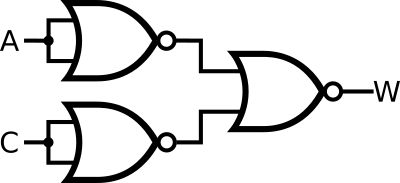
\includegraphics{w}
    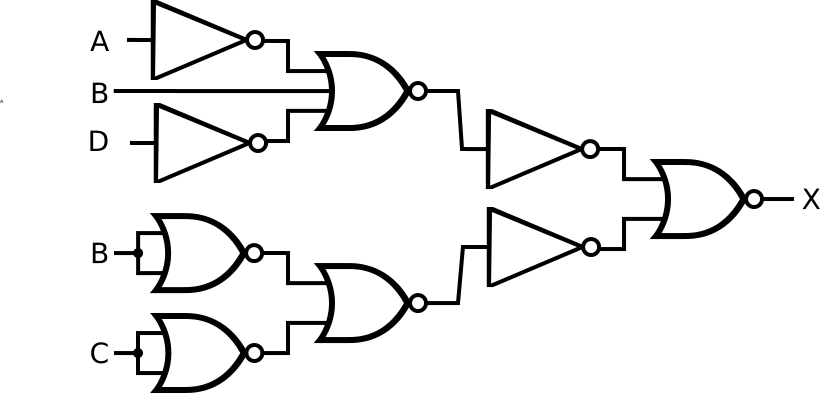
\includegraphics{x}
    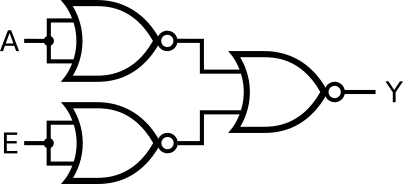
\includegraphics{y}
    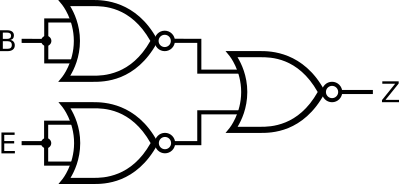
\includegraphics{z}
 
\end{document}
